\documentclass[10pt,journal,compsoc]{IEEEtran}

\usepackage[pdftex]{graphicx}
\usepackage{cite}
\hyphenation{op-tical net-works semi-conduc-tor}


\begin{document}

\title{Using Deep Neural Networks for autonomus drone navigation in orchard enviroiment}

\author{BRESILLA, Trim}

\markboth{Inference project, Robotic Nanodegree, Udacity}%
{}
\IEEEtitleabstractindextext{%

\begin{abstract}
With the increase of population in the world, the demand for quality food is increasing too. One of the biggest and the base of raw food production comes frim Agriculture. In the recent years, due to this demand, and other enviroimental factors have havily influenced the way agricultural production is done. Automation and robotics for fruit and vegetable production and monitoring has become the new standard.
\end{abstract}

\begin{IEEEkeywords}
Robot, IEEEtran, Udacity, \LaTeX, deep learning.
\end{IEEEkeywords}}


\maketitle
\IEEEdisplaynontitleabstractindextext
\IEEEpeerreviewmaketitle
\section{Introduction}
\label{sec:introduction}

\IEEEPARstart{T}{he} introduction should provide some material regarding the history of the problem, why it is important and what is intended to be achieved. If there exists any previous attempts to solve this problem, this is a great place to note these while conveying the differences in your approach (if any). The intent is to provide enough information for the reader to understand why this problem is interesting and setting up the conversation for the solution you have provided
Despite computers shrinking in size and increasing in performance, using them in the field has proven still to be not very cost effective. However lately with the increase of Neural Network, those tiny coputers are capable of doing better and more accurate calculations.
Use this space to introduce your robotic inference idea and how you wish to apply it. 
If you have any papers / sites you have referenced for your idea, please make sure to cite them.

%IMAGE
\begin{figure}[thpb]
      \centering
      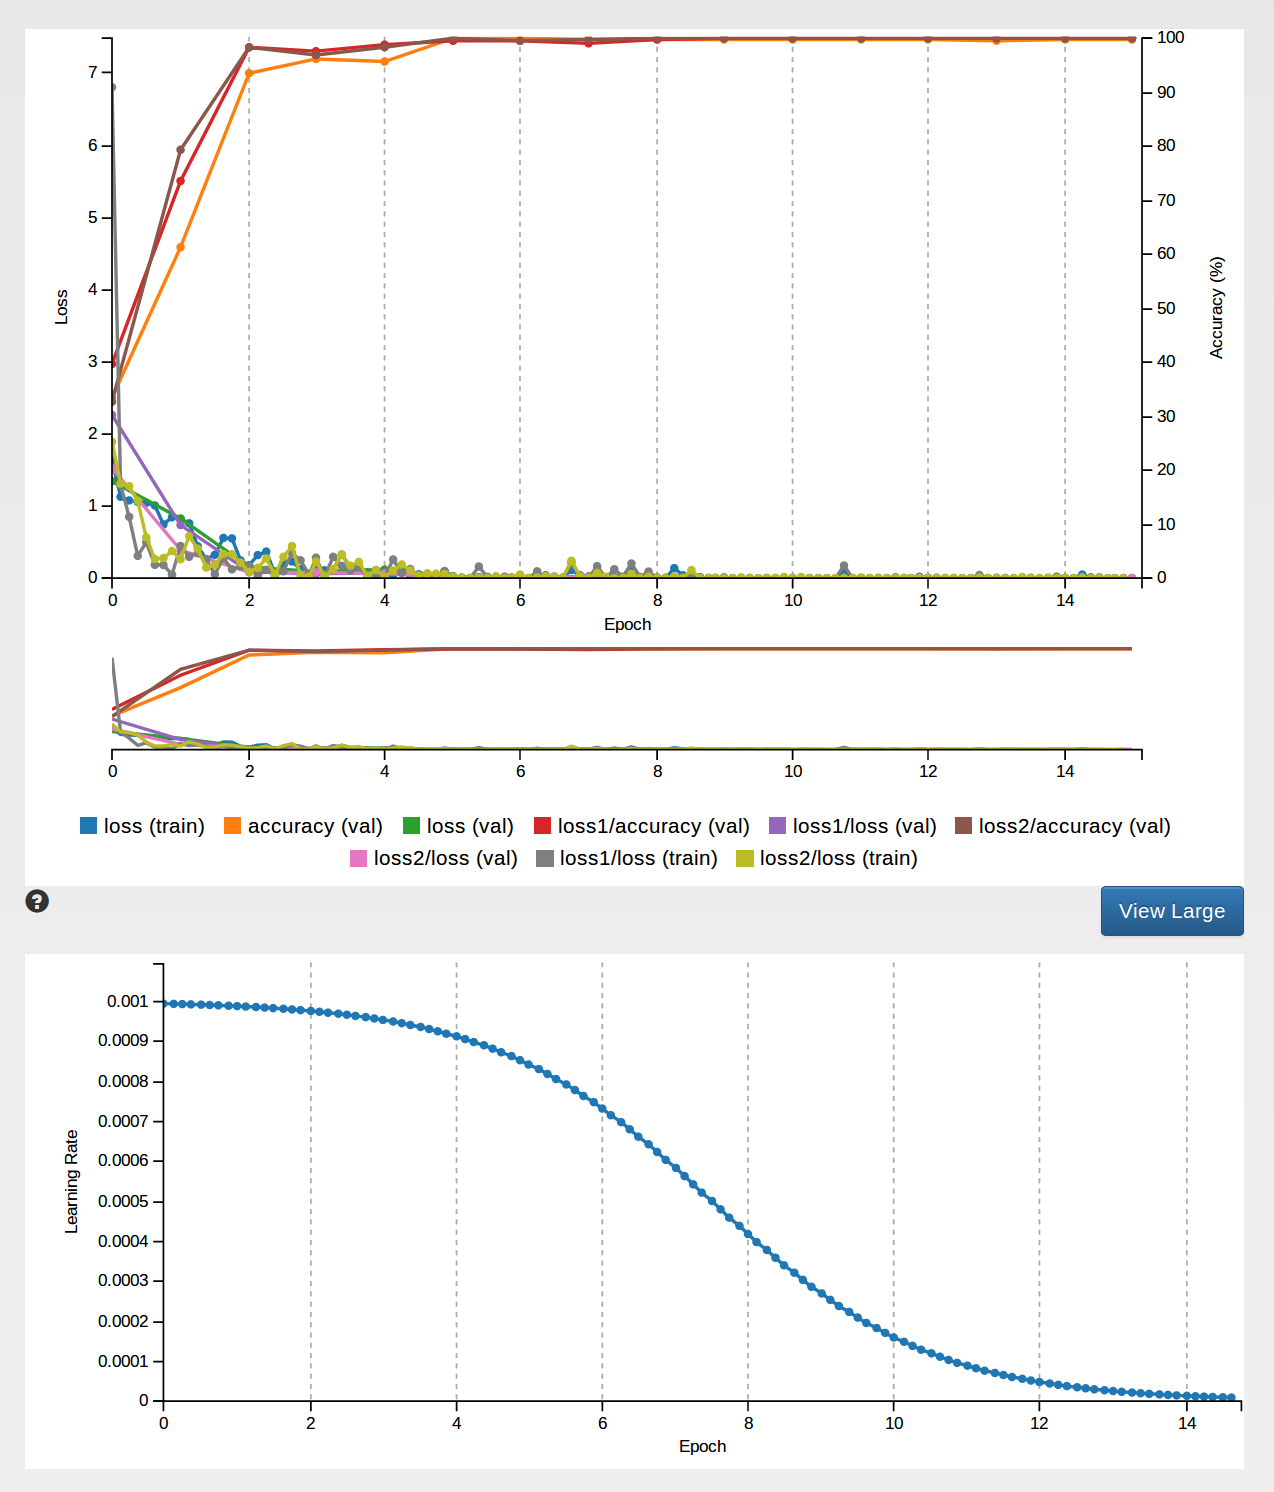
\includegraphics[width=\linewidth]{15_epoch_googlenet_sigmoidecay}
      \caption{Robot Revolution.}
      \label{fig:robot1}
\end{figure}

\section{Background / Formulation}
At this stage, you should begin diving into thththhe technical details of your approach by explaining to the reader how parameters were defined, what type of network was chosen, and the reasons these items were performed. This should be factual and authoritative, meaning you should not use language such as “I think this will work” or “Maybe a network with this architecture is better..”. Instead, focus on items similar to, ”A 3-layer network architecture was chosen with X, Y, and Z parameters” 
Explain why you chose the network you did for the supplied data set and then why you chose the network used for your robotic inference project. \cite{lamport1994latex}


\section{Data Acquisition}
This section should discuss the data set. Items to include are the number of images, size of the images, the types of images (RGB, Grayscale, etc.), how these images were collected (including the method). Providing this information is critical if anyone would like to replicate your results. After all, the intent of reports such as these are to convey information and build upon ideas so you want to ensure others can validate your process.
Justifying why you gathered data in this way is a helpful point, but sometimes this may be omitted here if the problem has been stated clearly in the introduction.
It is a great idea here to have at least one or two imagees showing what your data looks like for the reader to visualize.

\section{Results}
This is typically the hardest part of the report for many. You want to convey your results in an unbiased fashion. If you results are good, you can objectively note this. Similarly, you may do this if they are bad as well. You do not want to justify your results here with discussion; this is a topic for the next session. 
Present the results of your robotics project model and the model you used for the supplied data with the appropriate accuracy and inference time
For demonstrating your results, it is incredibly useful to have some charts, tables, and/or graphs for the reader to review. This makes ingesting the information quicker and easier.

\section{Discussion}
This is the only section of the report where you may include your opinion. However, make sure your opinion is based on facts. If your results are poor, make mention of what may be the underlying issues. If the results are good, why do you think this is the case? Again, avoid writing in the first person (i.e. Do not use words like “I” or “me”). If you really find yourself struggling to avoid the word “I” or “me”; sometimes, this can be avoid with the use of the word “one”. As an example: instead of : “I think the accuracy on my dataset is low because the images are too small to show the necessary detail” try: “one may believe the accuracy on the dataset is low because the images are too small to show the necessary detail”. They say the same thing, but the second avoids the first person. 
Reflect on which is more important, inference time or accuracy, in regards to your robotic inference project.

\section{Conclusion / Future work}
This section is intended to summarize your report. Your summary should include a recap of the results, did this project achieve what you attempted, and is this a commercially viable product? 
For Future work,address areas of work that you may not have addressed in your report as possible next steps. For future work, this could be due to time constraints, lack of currently developed methods / technology, and areas of application outside of your current implementation. Again, avoid the use of the first-person.

\bibliography{bib}
\bibliographystyle{ieeetr}

\end{document}
